\chapter{Introduction}
\label{Introduction}

% Define some commands to keep the formatting separated from the content 
\newcommand{\keyword}[1]{\textbf{#1}}
\newcommand{\tabhead}[1]{\textbf{#1}}
\newcommand{\code}[1]{\texttt{#1}}
\newcommand{\file}[1]{\texttt{\bfseries#1}}
\newcommand{\option}[1]{\texttt{\itshape#1}}

Predicting the outcome of sports matches has become a popular application of machine learning algorithms \cite{mlsports}. \textit{Esports} are video games which are played in a competitive setting. The games and their associated competitions are becoming increasingly popular; in 2021 the   

\section{Background and context}

\subsection{Evolution of Esports}

Competitive gaming started in the 1970s and 80s on the floors of public arcades. The best players would rise to the top of  high-score leaderboards in their favourite titles like \textit{Space Invaders}, \textit{Pac-Man}, and \textit{Tetris}. This type of competition was indirect, but by the 1990s, multi-player fighting games like \textit{Street Fighter} would see players pitted directly against each other. By then, the transition from arcades floors to home consoles and PCs was well under way, and the LAN party became the new battle arena. \textit{Doom} and \textit{Quake} marked the rise of first-person shooters (FPS) in this era. At the dawn of the 2000s, real-time strategy (RTS) games like \textit{StarCraft} and \textit{Warcraft} spawned the first professional leagues, legitimizing competitive gaming.

High-speed internet became ubiquitous by the 2010s, and esports went mainstream. Multiplayer online battle arena (MOBA) games like League of Legends and Dota 2 rose to prominence, and now boast tournaments with multi-million dollar prize pools. The esports betting industry developed in a similar fashion; projections of the total amounts wagered on esports far exceed the revenues generated by the competitions themselves. 

Today there are a substantial variety of game genres that are played professionally across the globe. Viewership figures for the major tournaments already rival traditional sports, and esports continue to grow and evolve without any showing any signs of slowing down. \cite{proesports-book}

\subsection{Introduction to Counter-Strike}

\subsubsection{Counter-Strike as an Esport}

Counter-Strike first emerged in 1999 as a 'mod' (modification) for the hit FPS by Valve Corporation, \textit{Half-Life}. The following year, Valve hired the developers of the mod, acquired the IP, and subsequently launched Counter-Strike as a standalone title. It didn't take long for a competitive scene to emerge. The first tournaments were organized in Europe by the Cyberathlete Professional League (CPL), with humble prize pools of ten to twenty thousand euros. Since then, the game has soared in popularity over a number of iterations, and the quality and scale of competition has grown along with it. 

Today there are several competitive leagues hosted by organizations like ESL, DreamHack, and Intel Extreme Masters. These leagues typically culminate in major LAN events, where the top teams compete for the lion share of prize pools which can exceed a million dollars. Valve-sponsored Major tournaments represent the pinnacle of the CS calendar, and attract millions of concurrent viewers on streaming platforms in addition to a packed stadium of fans. Top players, like  Nicolai 'device' Reedtz from Denmark and Gabriel 'FalleN' Toledo from Brazil, are considered national celebrities.

\subsubsection{Counter-Strike Fundamentals}

Counter-Strike is a PC video game played using the mouse, keyboard, and microphone. Players assume the role of a soldier in a virtual 3D environment. In terms of movement, players can run, walk, and jump by pressing keys on the keyboard. Aiming is performed by moving the mouse, which moves the player's field-of-vision in-game. Players co-ordinate their actions with their team primarily through voice communication. 

Although a number of versions have been released since its inception, the core game mode played in Counter-Strike, known as 'defusal', has remained relatively unchanged. Two teams of five players each start each round on opposite ends of an arena called a 'map'. One team plays the role of the Counter-Terrorists (CT), whose objective is to defend two bomb sites, A and B, from the opposing team, the Terrorists (T). The layout for the most popular Counter-Strike map in competitive play, Mirage, is shown in Figure \ref{fig:mirage}; the red zones highlight the bomb sites and the green zones are the spawn areas for either team.

In each round of play, each player has only one life, and if eliminated, must spectate their living team-mates until the round concludes. Teams can win rounds either by (1) eliminating the entire enemy team, or, if playing as Terrorists (T), by (2) detonating a bomb on one of the bomb sites. The Counter-Terrorists (CT) can win rounds either by (3) successfully defending both sites for the duration of the round, or by (4) defusing the bomb after it has been planted. Players start each round with 100 health points (HP). Damage can be inflicted using a variety of weapons and grenades. There is no way to replenish HP during a round.

\begin{figure}[h]
	\centering
	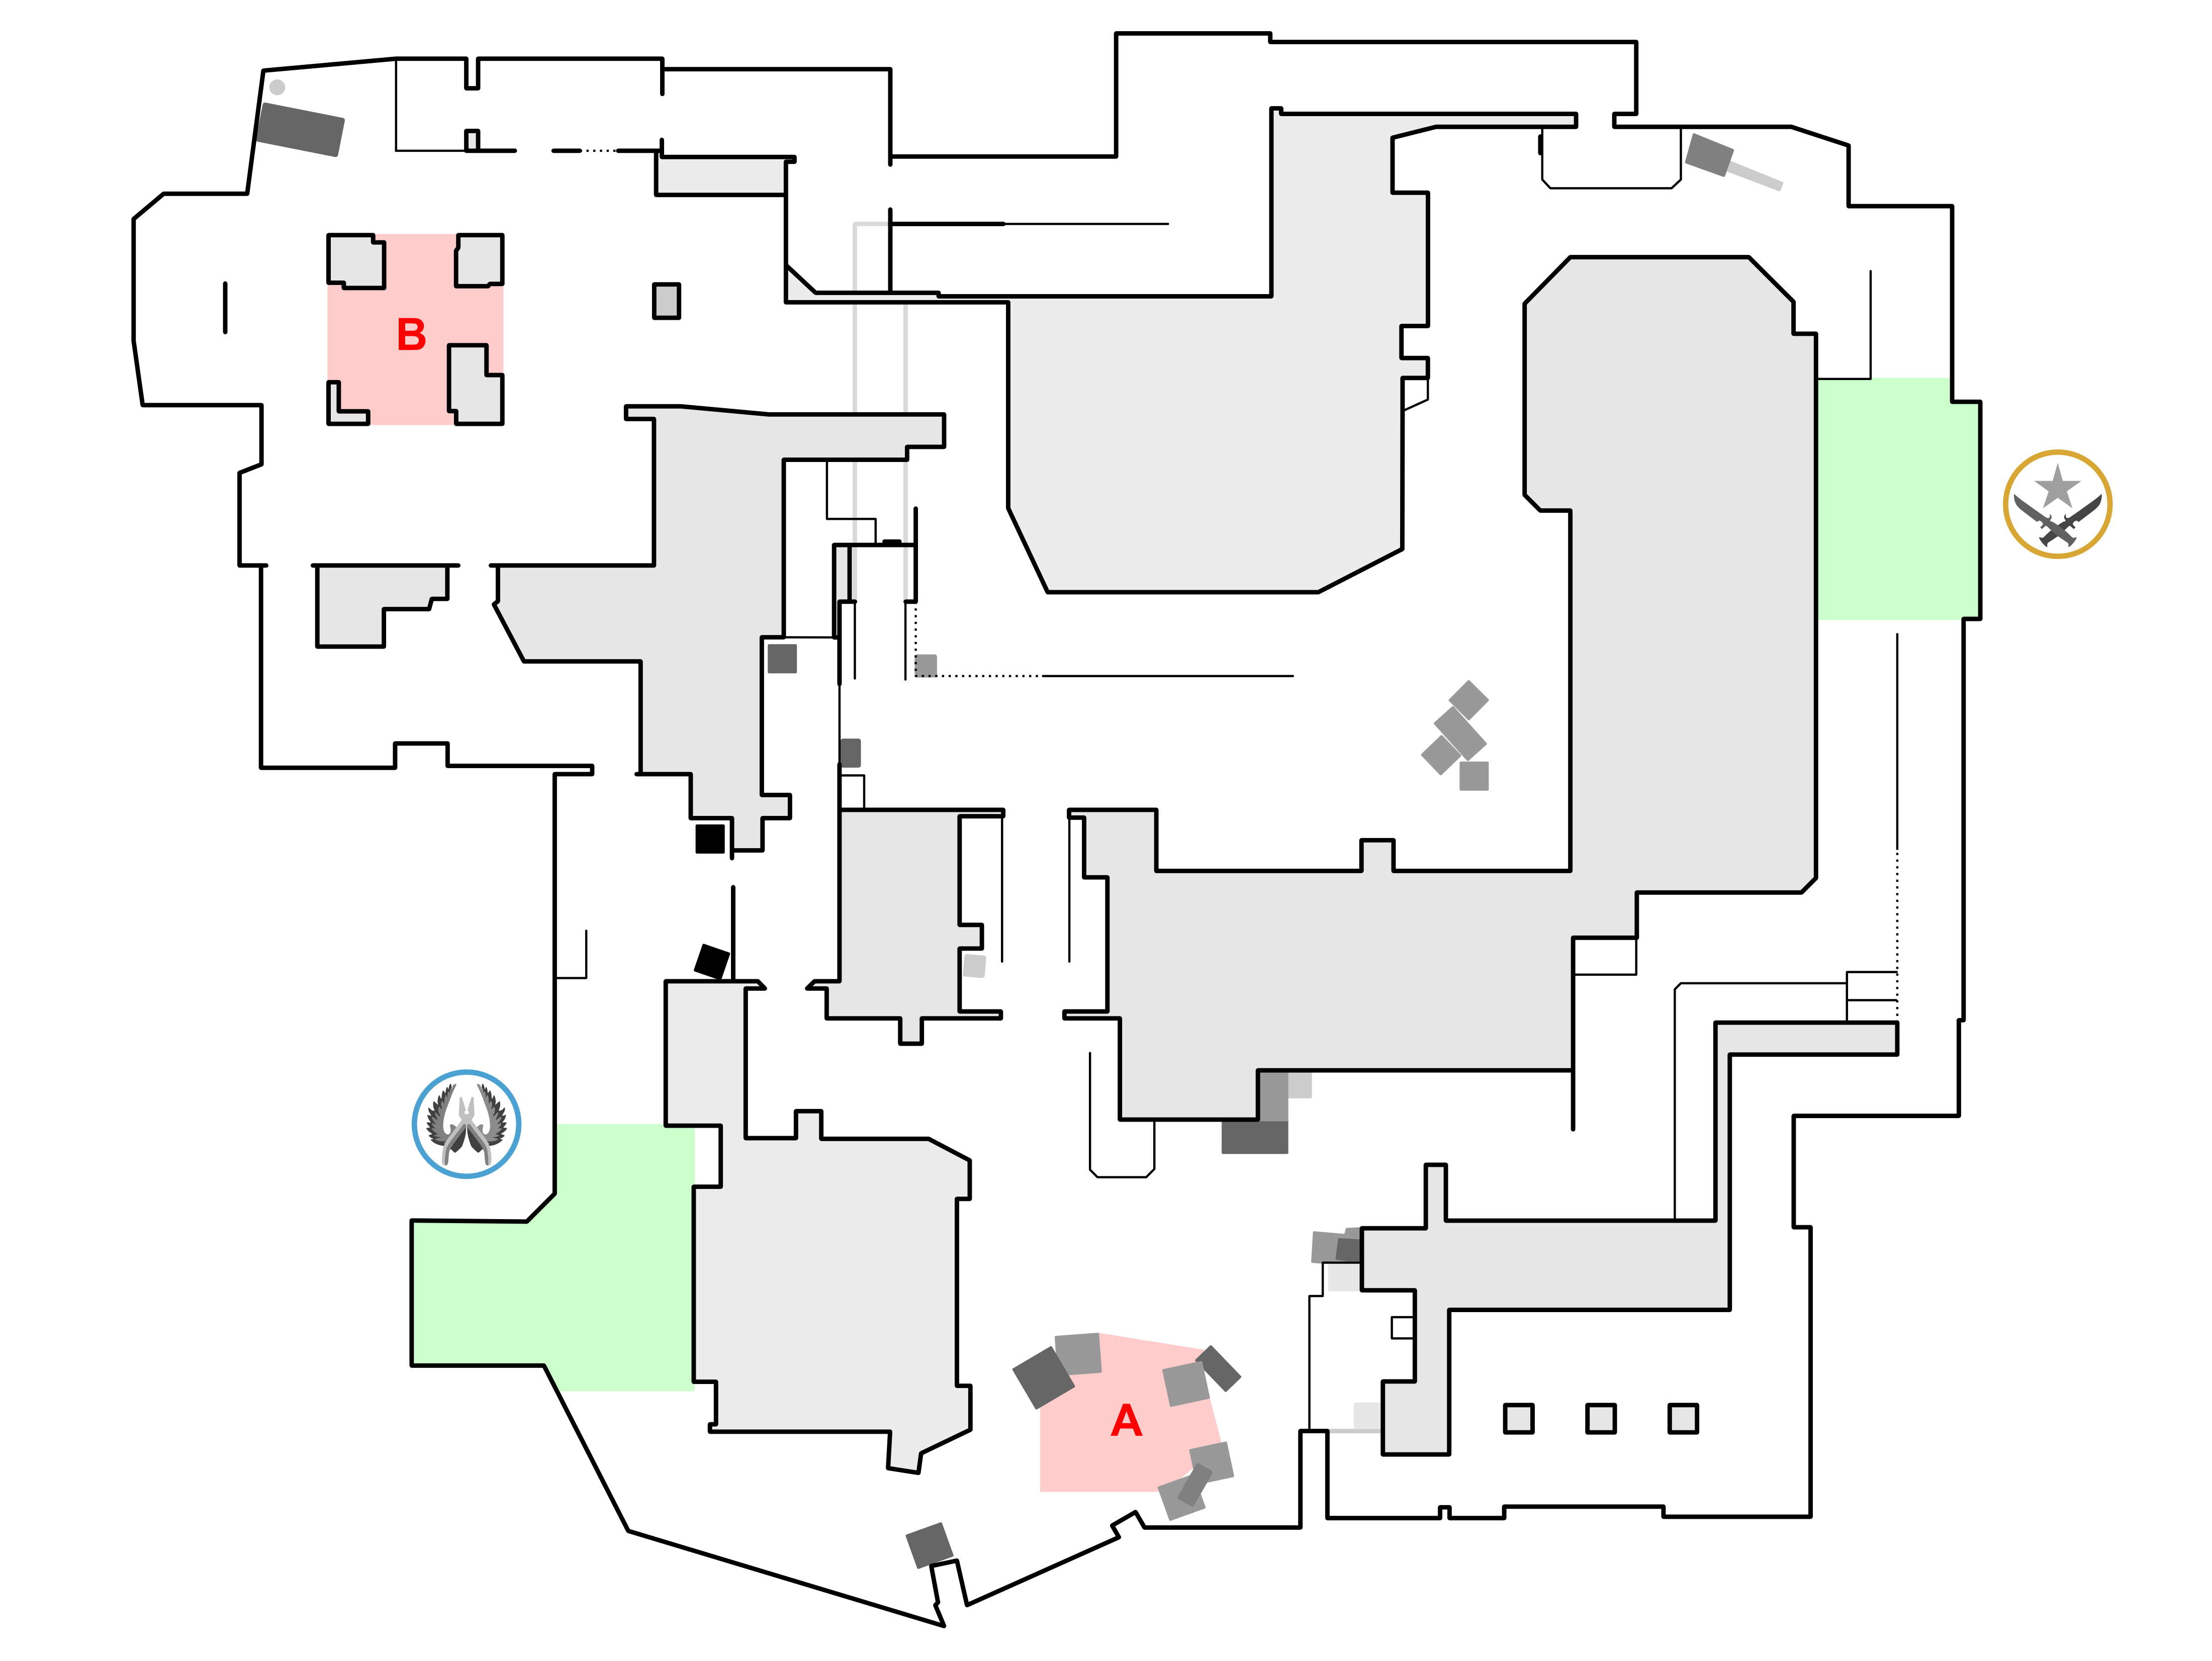
\includegraphics[width=0.9\textwidth]{Figures/mirage.png}
	\caption{Map layout for 'Mirage', showing spawn areas and bomb sites}
	\label{fig:mirage}
\end{figure}

Players are rewarded with in-game money for getting a kill, planting or defusing the bomb, and winning or losing a round. Winning a round is rewarded with far more money than losing a round, however this amount (the 'loss bonus') grows with each consecutive round loss. Money is spent to purchase weapons and equipment at the start of each round. If a player survives the round, they retain whatever equipment they had into the following round. Each team therefore has an 'economy' which fluctuates throughout the duration of a map. A stronger economy means you can purchase stronger weapons and more equipment. A weaker economy might relegate your team to just buying a few pistols and practically forfeiting a round in order to save funds for the following round. Sound economic strategy is thus critical to success in Counter-Strike.

At the start of a half, both sides have almost no money and so duel with only pistols. The 'pistol round' is quite crucial, as it initiates economic momentum for whichever team wins it. In some exciting cases, teams will defy odds and trade the initial rounds back-and-forth, leaving the economic balance undecided. A game can become extremely tense if both teams have precarious economies near the end, as the outcome is undecided and the stakes get progressively higher. 

An example of the economy in a map of Counter-Strike is shown in Figure \ref{fig:economy} below. The coloured icons represent a round won by the CTs (blue) or the Ts (orange). The pistol rounds take place in rounds 1 and 13. The y-axis represents the sum of the value of the equipment purchased by either team in each round.

\begin{figure}[h]
	\centering
	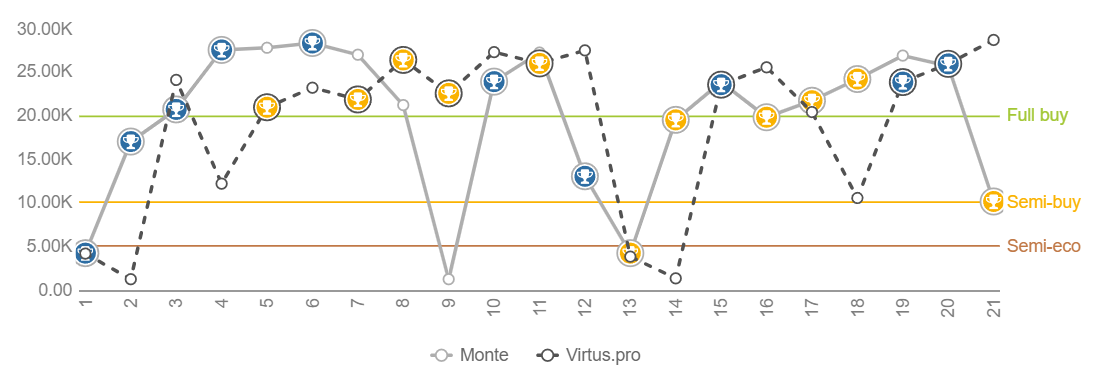
\includegraphics[width=\textwidth]{Figures/economy.png}
	\caption{A graph showing the economies of two teams over the course of a map}
	\label{fig:economy}
\end{figure}

There are seven maps in the 'map pool'. This is analogous to the circuit of race tracks in a season of Formula 1. Each map is played for best-of-24 rounds, with teams swapping sides after 12 rounds. This means that in order to win, teams must demonstrate both a superior T-side and CT-side than their opponents. The first team to reach 13 round wins takes the map point. If the score ends in a tie (12-12), the map continues in best-of-6 round overtimes until a winner is decided.

Different strategies ('meta's) evolve for attacking and defending the various points on each map, with players learning which positions are optimal to hold with different weapons, when and where to throw "utility" (smoke, flash-bang, high-explosive, and incendiary grenades), and how to rotate players around the map as the round unfolds. All positions on a given map are named such that players can immediately communicate critical gameplay information to their teammates over the course of a round.

\subsubsection{Competitive Counter-Strike}

Counter-Strike matches are typically played in a best-of-1 (BO1) or best-of-3 (BO3) maps format. Grand finals are often contested in a best-of-5 (BO5) map series. Match lengths can vary greatly depending on the format and skill-disparity between competitors. A lopsided BO1 can be 20-minute 13-0 thumping. In extreme cases, a BO5 grand final between two evenly-matched giants can become a gruelling five-hour affair as tightly-contested maps get traded back-and-forth. The most common format is the BO3, where a match is determined over 2 or 3 maps which last roughly 40 minutes each.

Although CS is a methodical and tactical team-based shooter, it is highly dynamic in the short, medium, and long term. During individual rounds, players must make split-second decisions to react to events as they unfold. Over the course of a map of 24 rounds, teams need to learn and adapt to their opponent's habits in order to exploit their weaknesses. And between matches, teams often adopt and improve on other team's strategies by reviewing their gameplay demos, or come up with entirely new approaches to counter a certain prevailing strategy.  

Teams also have coaches whose role is to identify these trends on the fly and suggest appropriate countermeasures. The best teams employ analysts for the same purpose. Competitive CS is heavily mentally demanding, so teams often have sports psychologists to keep the players' operating at peak performance. During the match, coaches need to keep the players in check to avoid 'tilting' - getting frustrated when losing badly, or getting overconfident when things are going well.


\subsubsection{Data in Counter-Strike}

Every second of CS game play generates a wealth of information; the 'tick rate' is the frequency at which each player's game client is synchronized with the server. Professional matches are played exclusively on '128-tick', which means there are 128 new dataframes being generated per second containing every minute detail of the game: each player's precise location on the map, the direction at which they are aiming, and the state they are currently in - moving, jumping, shooting, throwing a grenade, reloading, switching weapons, planting or defusing a bomb, shooting or being shot at. At any given point there can be a number of smoke grenades deployed on a map, a high-explosive grenade being lobbed towards an enemy position, or a incendiary grenade temporarily blocking a choke point.

Each round is 1 minute 55 seconds; this is the time in which the Ts have to take control of either site and plant a bomb. Once planted, there are 40 seconds until detonation. The CTs must 'retake' the site and defuse the bomb before this happens in order to win the round. Multiply the tick rate by the average round time and then again by the number of rounds and it should be evident that there is a tremendous amount of data generated in each map played. This data is serialized into a 'demo-file' which is often compressed into 32- or 64-tick.

The state of each team's economy gives a clear indicator of their ability to win a given round. This is the total team balance as well as their current loss bonus; teams earn progressively more money with consecutive round losses up to a cap of \$3400 after 5 losses in a row - matching the round-win bonus. A team with the funds to 'full-buy' will almost always win a round against a team that is saving in an 'eco' round. A 'semi-buy' leaves enough funds to ensure a 'full-buy' the following round, and gives the team a fighting chance at least.

Player performance can be measured with many metrics: player kills, deaths, assists, average damage per round (ADR), and weapon accuracy are all highly relevant. Online tools like Leetify also extract more metrics from demo-file data: cross-hair placement refers to the degree deviation of the cursor from an enemy who comes into view, time-to-damage is the milliseconds between seeing an enemy and inflicting damage, headshot accuracy is the proportion of hits that are to the enemy's head, and reaction speed is the number of milliseconds before reacting to an enemy coming into view. 'Clutch' statistics refer to the percentage of rounds won where a player is last alive on his team versus 1, 2, 3, 4, or 5 opponents. All of these data points, and more, paint a descriptive picture of a player's contribution to their team's success, or defeat. That said, some roles, such as 'support' or 'in-game leader' (IGL) help their team in ways that are harder to quantify.

Team performance is usually measured by their win-rates on the various maps. Teams have preferred maps, and most also have 'perma-bans' which they never play. In a BO3 series, teams will decide which of the 7 maps to play through a veto process; this follows a ban-ban-pick-pick-ban-ban-decider sequence. There are therefore trends in which maps a team will play and will avoid. A map-veto which favours one team in an otherwise equal match-up can therefore make for a favourable bet.

All these statistics are prominent features of a professional broadcast; for example, commentators will refer to the weapon accuracies when contrasting the snipers of opposing teams. Dominant teams can go on significant match or map-win streaks, which adds further tension to tight matches. On certain broadcasts, there is a round-win prediction percentage which sways depending on the round economy and number and health of players alive on each side.

\subsection{Challenges in Counter-Strike Match Prediction}

\subsection{Overview of Machine Learning Techniques}

\section{Research problem}

\section{Research objectives}

The primary objective of this research is to predict the winner of professional Counter-Strike matches by employing machine learning techniques. This can be achieved by means of the following research objectives:

\begin{enumerate}
	\item \textbf{Predict Map Selection}\\
	The majority of professional Counter-Strike matches are played in the best-of-3 (BO3) maps format. There are seven maps in the competitive map pool. The first step is to predict which maps will be banned and picked by either team during the pre-match map selection process (also referred to as "the veto").
	\item \textbf{Predict Map Winners}\\
	A team's proficiency varies from map to map. The second step is to predict the winner of each map for any permutation of the veto process.
	\item \textbf{Predict Overall Winner}\\
	The final step is to combine the outputs of the map-veto prediction and the map-winner predictions into an overall match win probability.
\end{enumerate}

\subsection{Methodology}

To accomplish these objectives, the research will follow a structured methodology:

\begin{enumerate}
	\item \textbf{Data Collection}\\
	Collect a large dataset of professional Counter-Strike match records and statistics.
	\item \textbf{Data Analysis}\\
	Find trends in the collected data to inform feature engineering and the development of heuristic baseline predictions (for example, "the higher-ranked team always wins" and "the team with the higher win-rate on the three maps always wins")
	\item \textbf{Feature Engineering}\\
	Generate relevant features from the dataset by processing the match and map records. These features can include team-based features, such as 'recent map win-rate', and player-based features such as 'average KDR'.
	\item \textbf{Modelling}\\
	Employ a series of classification models (logistic regression, gradient-boosted decision trees, and neural networks) on the dataset.
	\item \textbf{Performance Analysis}\\
	The performance of each model will be measured by means of classification accuracy, precision, recall, F1-score, and AUC-ROC. The models will be compared to one another as well as to the baseline performance achieved by the heuristic predictions discussed above. 
\end{enumerate}


\section{Significance of the study}

The consequences of this research bears significance to a number of stakeholders:
\begin{itemize}
	\item Betting Industry\\
	Both \textbf{bookmakers} and \textbf{bettors} can benefit from this research; bookmakers can improve the accuracy of their odd-setting, while betters can potentially improve their profitability by implementing the insights into their own betting strategies. This research could contribute to betters making more informed decisions, thereby promoting responsible betting.
	\item Esports Community\\
	Professional teams (\textbf{players}, \textbf{coaches}, and \textbf{analysts}) can improve their strategies and training regimes to optimize their statistical likelihood of success.
	\item Viewer Experience\\\textbf{Commentators} can colour in compelling story lines with statistics. \textbf{Broadcasters} can enhance their streams by incorporating data-driven insights, potentially improving viewer engagement. \textbf{Counter-Strike fans} may find entertainment value from a deeper understanding of match predictability.
	\item Tournament Organizers\\
	Predictive information can assist \textbf{tournament organizers} to structure their tournaments and schedules in order to maximize the competitive fairness of their tournaments. They could also be used to design fair qualification systems or choose which teams to invite.
	\item Academia\\
	This research contributes to the understanding of esports betting and predictive modelling of professional Counter-Strike. \textbf{Future researchers} may find it to be a valuable resource for further study into these topics.
	
\end{itemize}

\section{Scope and limitations}

Every sport possesses a degree of inherent unpredictability; this is a large part of what makes spectating a match enjoyable. Professional Counter-Strike is no different to football or chess in this regard. The accuracy of predictive models are thus subject to the quality of the available data and the modelling techniques employed.

\section{Structure}

This paper is split into five chapters.

The introduction covers some essential background, defines the research problem, and establishes the objectives. The literature review provides a summary of the existing research on esports betting and data-driven prediction. 

The third chapter describes the methodology employed: describes how the data was collected, stored, processed, analysed, and converted into features.  The dataset is then used to train an ensemble of machine learning models. 

The penultimate chapter is a discussion of the results. Finally, a conclusion summarizes the key findings, and suggests areas worth researching further.

% Notes

%1. What will you research? (research topic)
%2. Why is that important? (justification)
%3. Scope
%4. Limitations
%
%1. Opening section: introduce reader to research in high level terms
%2. Study background: context of project
%3. Research problem: gap that exists in current research
%4. Aims, Objectives, and Questions
%5. Significance, why is it worth doing, what value does it provide to the world
%6. Limitations of project and approach
%7. Structure


